\documentclass{aa}

\usepackage{graphicx}
\usepackage{amsmath}
\usepackage{hyperref}
\usepackage{url}

\begin{document}

\title{GASP: A Corrected, Cross-Matched Catalog of 19\,190
       Gaia DR3 Asteroid Reflectance Spectra}

\author{W.~Scheibenpflug\thanks{wscheibenpflug@gmail.com}}

\institute{Independent researcher, Vienna, Austria}

\abstract
{Gaia Data Release 3 (DR3) provides mean reflectance spectra for 60\,518
Solar System objects, but carries a systematic near-ultraviolet (NUV)
artifact and no corrected, cross-matched catalog was publicly available.}
{I present GASP (Gaia Asteroid Spectral Pipeline), an open-source pipeline and
catalog of NUV-corrected Gaia DR3 asteroid reflectance spectra enriched with
ancillary photometric and physical data.}
{I download 968\,288 spectral measurements from the Gaia Science Archive,
apply the NUV correction of \citet{TinautRuano2023}, and cross-match on MPC
asteroid number with the SDSS Moving Object Catalog (MOC4), the
\citet{Nesvorny2015} HCM family catalog, NEOWISE albedos, and the
\citet{Mahlke2022} spectral taxonomy.}
{The catalog contains 19\,190 asteroids with 16-band NUV-corrected spectra
(374--1034~nm), SDSS $a^*$ colors, NEOWISE albedo (22.3\%), family
membership (39.3\%, 117 families), MPC orbital classification (100\%), and
spectral slopes $s_1$--$s_4$. Cross-validation against the Eight Color
Asteroid Survey \citep[ECAS;][]{Zellner1985} yields Pearson $r = -0.848$
($n = 83$, $p \approx 0$), confirming consistency with ground-based
photometry.}
{GASP provides two complementary spectrophotometric discriminators --- NUV
slope and SDSS $a^*$ color --- in a single, consistently processed dataset.
The catalog and reproducible pipeline are publicly available on GitHub and
Zenodo (\href{https://doi.org/10.5281/zenodo.19366681}{10.5281/zenodo.19366681}).}

\maketitle

\keywords{minor planets, asteroids: general -- catalogs --
techniques: photometric -- surveys}

\section{Introduction}

The third data release of the ESA Gaia mission
\citep[Gaia DR3;][]{GaiaDR3_2023} includes mean reflectance
spectra for 60\,518 Solar System objects (primarily asteroids)
across 16 wavelength bands between 374 and 1034~nm. Despite
their scientific potential, these spectra carry a known
systematic artifact: an artificial reddening below 0.55~$\mu$m
caused by inadequate solar analogues in the near-ultraviolet
\citep[NUV;][]{TinautRuano2023}. No publicly available,
corrected, and cross-matched catalog existed prior to this work.
The reproducible processing pipeline and the resulting catalog are
archived on Zenodo \citep{scheibenpflug_2026_gasp}.

\section{Pipeline}

GASP consists of eight Python scripts executing sequentially.
Starting from the Gaia Science
Archive\footnote{\url{https://gea.esac.esa.int/archive/}}
\citep{Galluccio2023},
I download 968\,288 rows (60\,518 asteroids $\times$ 16 spectral
bands) and restructure them into wide format (one row per asteroid).
I apply the NUV correction of \citet{TinautRuano2023}, dividing
reflectance values at 374, 418, 462, and 506~nm by factors of
1.07, 1.05, 1.02, and 1.01, respectively (their Table~1).

Cross-matching with the Sloan Digital Sky Survey Moving Object
Catalog \citep[SDSS MOC4;][]{Ivezic2001} on MPC asteroid number
yields 19\,190 objects present in both surveys (31.7\% of the
full Gaia SSO catalog). The inclusion of SDSS $a^*$ colors
enables a robust, independent check of C- vs.\ S-complex
separation; combined with the NUV-corrected Gaia slopes, GASP
provides two complementary spectrophotometric discriminators for
asteroid surface composition in a single, consistently processed
dataset.

I further enrich this sample with family membership from the
\citet{Nesvorny2015} HCM catalog (PDS4 archive V2.0, 117
families), spectral taxonomy from \citet{Mahlke2022}, albedo and
diameter from NEOWISE \citep{Masiero2011}, and orbital
classification from the MPC Extended Object Catalog. Spectral
slopes $s_1$--$s_4$ (in $\mu$m$^{-1}$) are computed following
the methodology of \citet{TinautRuano2024}.

\section{Catalog properties}

The final catalog contains 19\,190 asteroids across 72 columns.
Family membership reaches 39.3\% (7\,533 objects in 117 families),
with the largest families being Nysa-Polana ($n = 3\,891$),
Vesta ($n = 2\,847$), and Flora ($n = 2\,156$). Spectral taxonomy
is available for 1.9\% of objects (358 asteroids), reflecting
the limited size of currently available ground-based spectral
classifications rather than a pipeline limitation. NEOWISE
albedo and diameter are available for 22.3\% of objects
(4\,286 asteroids). All 19\,190 objects carry MPC orbital
classification; 94.4\% are Main Belt Asteroids. Full catalog
statistics are available at the Zenodo repository
(DOI: \href{https://doi.org/10.5281/zenodo.19366681}%
{10.5281/zenodo.19366681}).

\section{Validation}

I validate the NUV correction by cross-matching my catalog
with the Eight Color Asteroid Survey
\citep[ECAS;][]{Zellner1985}, which provides ground-based
photometry in eight broadband filters including two below
0.45~$\mu$m. Of 589 ECAS asteroids, 83 appear in my catalog.
I compute the Pearson correlation between the ECAS $b-v$ color
index and the GASP reflectance at 418~nm (\texttt{refl\_418}),
the closest Gaia band to the ECAS $b$ filter (central wavelength
0.437~$\mu$m). I find $r = -0.848$ ($p \approx 0$, $n = 83$;
Fig.~\ref{fig:ecas}), confirming that the NUV-corrected Gaia
spectra are consistent with independent ground-based photometry.
The negative sign reflects the inverse relationship between
reflectance ratio and color index conventions.

Figure~\ref{fig:astar} shows the SDSS $a^*$ color index
\citep[a C/S-complex separator;][]{Ivezic2002} plotted
against the NUV slope $s_1$, colored by NEOWISE albedo.
C-complex asteroids ($a^* < -0.10$) show lower albedo
(mean $p_V \approx 0.06$) and more negative $s_1$ values,
consistent with hydrated, UV-absorbing primitive material.
S-complex asteroids ($a^* > 0.10$) show higher albedo
(mean $p_V \approx 0.22$) and flatter NUV slopes, consistent
with anhydrous silicate compositions.

\begin{figure*}
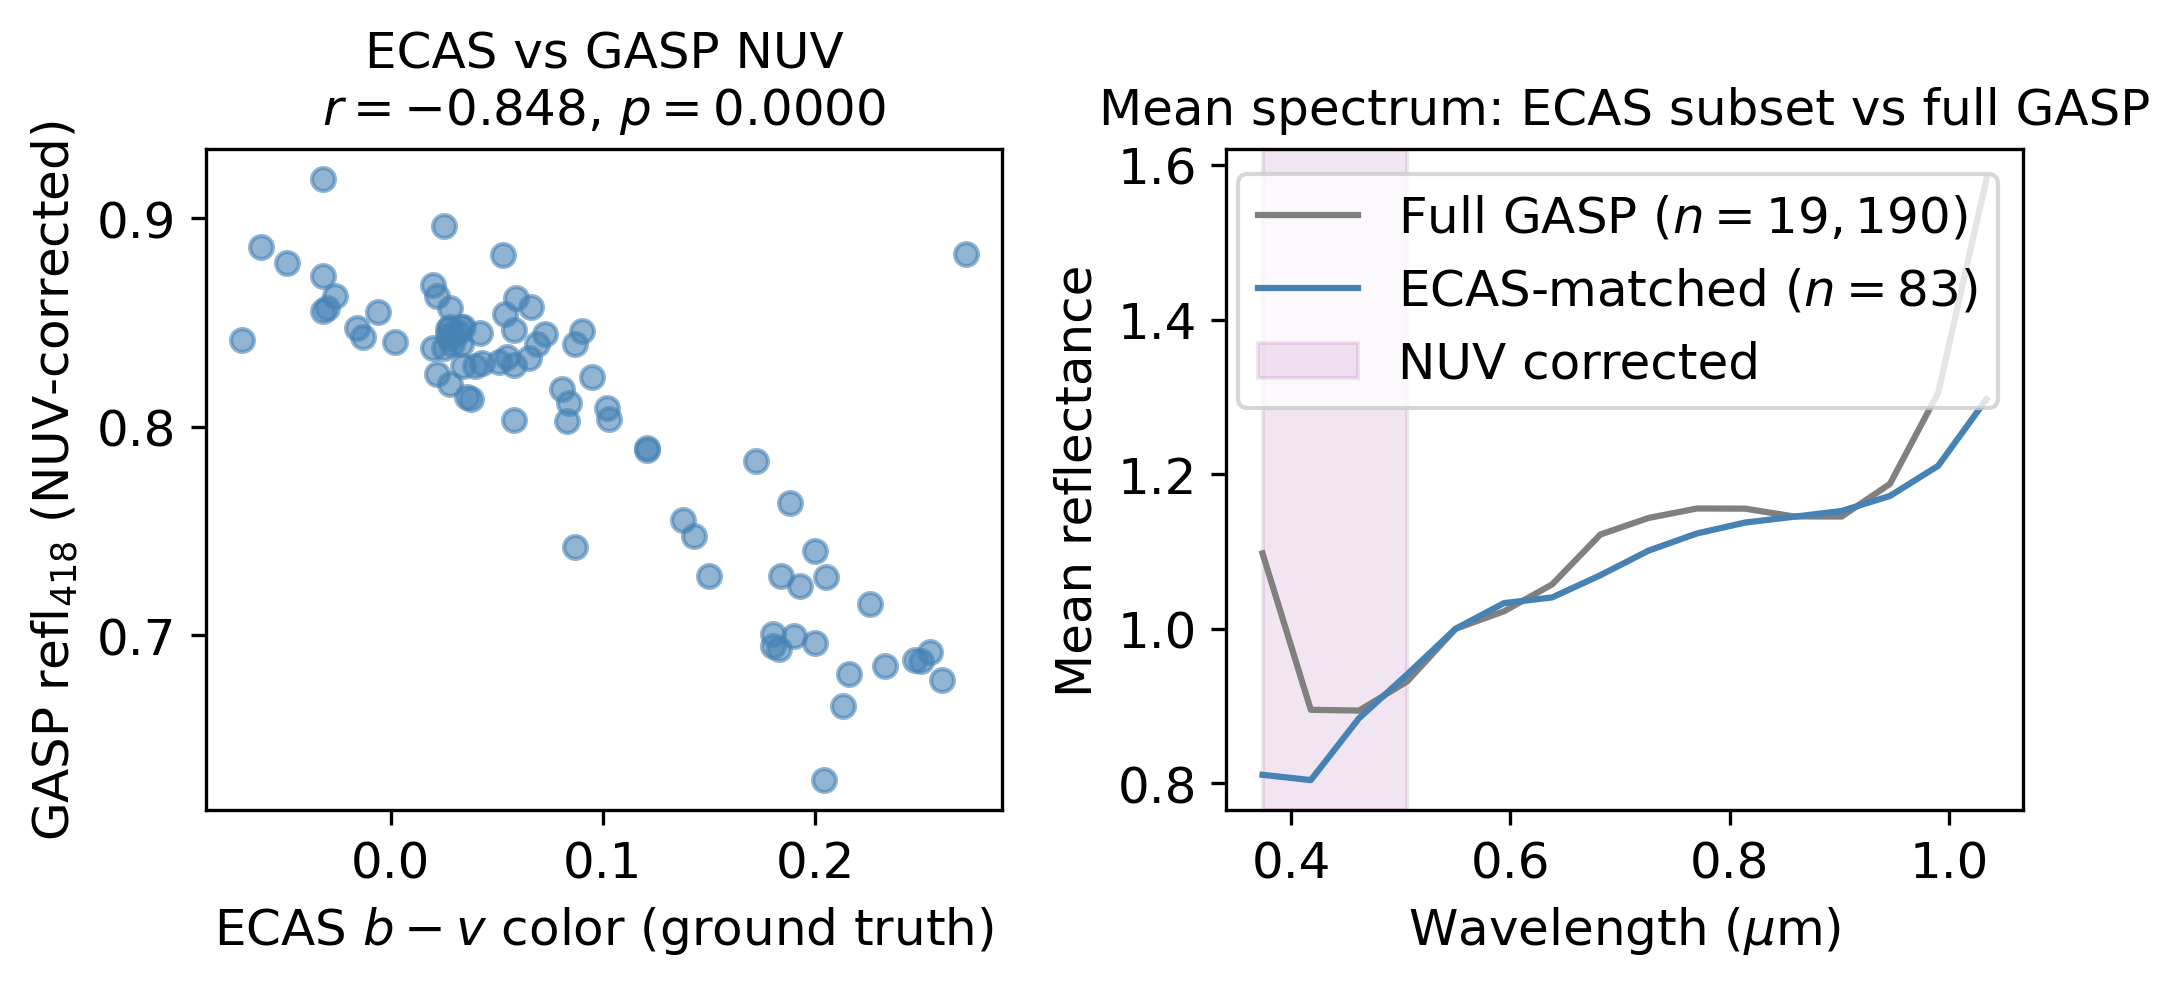
\includegraphics[width=\textwidth]{figures/05_ecas_validation.png}
\caption{Left: ECAS $b-v$ color vs.\ GASP \texttt{refl\_418}
(NUV-corrected reflectance at 418~nm) for the 83 asteroids
common to both catalogs. The strong negative correlation
($r = -0.848$, $p \approx 0$) confirms that the NUV correction
produces spectra consistent with ground-based photometry.
Right: Mean spectrum of the ECAS-matched subset compared to the
full GASP sample (gray), with the NUV-corrected region
highlighted (purple shading).}
\label{fig:ecas}
\end{figure*}

\begin{figure*}
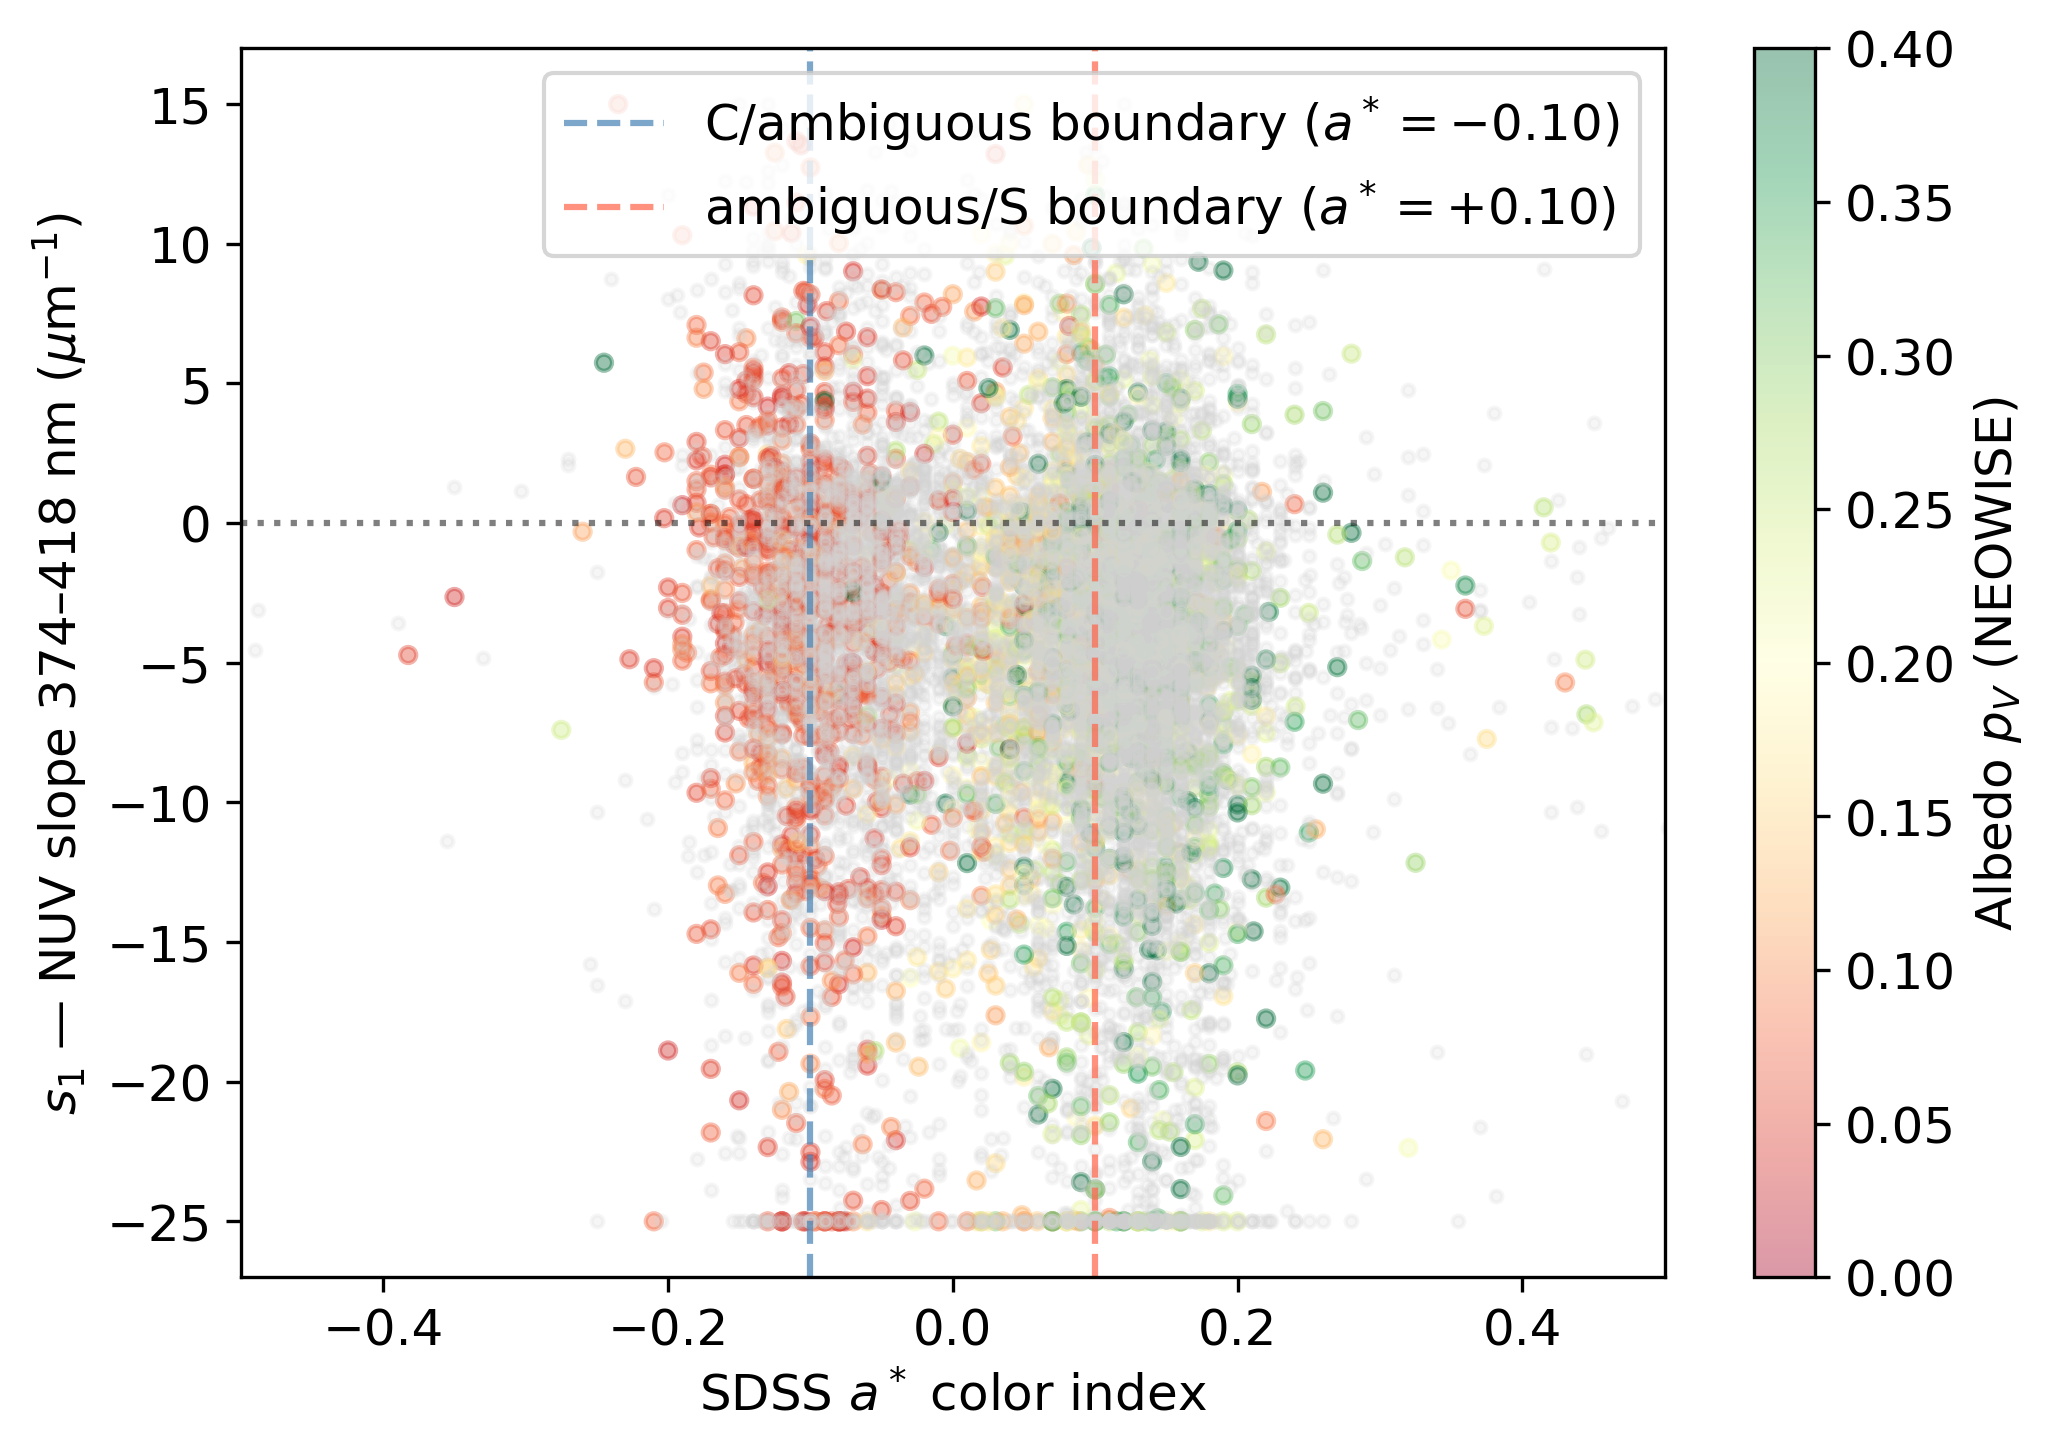
\includegraphics[width=\textwidth]{figures/03_astar_vs_s1.png}
\caption{SDSS $a^*$ color index \citep[C/S-complex
separator;][]{Ivezic2002} vs.\ NUV slope $s_1$
(374--418~nm) for all 19\,190 GASP asteroids with both
quantities available. Points are colored by NEOWISE albedo
($p_V$; 22.3\% of the sample; gray: no NEOWISE match).
Vertical dashed lines delineate the C-complex
($a^* < -0.10$), ambiguous, and S-complex ($a^* > 0.10$)
populations. C-complex objects show lower albedo
(mean $p_V \approx 0.06$) and more negative $s_1$;
S-complex objects show higher albedo
(mean $p_V \approx 0.22$) and flatter NUV slopes.}
\label{fig:astar}
\end{figure*}

\section{Limitations}

Taxonomy coverage reflects the current state of ground-based
spectral surveys, not a pipeline limitation. The SDSS MOC4
cross-match yields 31.7\% of the full Gaia SSO catalog;
objects without SDSS counterparts are available in the
intermediate pipeline output at the same Zenodo record.
A systematic reddening has been observed in Gaia DR3 SSO
spectra at wavelengths between 0.7 and 0.9~$\mu$m; a
peer-reviewed correction is not yet published, and this
NIR artifact is not corrected in GASP v1. This is planned
for a future release coinciding with Gaia DR4
(expected end of 2026).

\section{Data availability}

The complete catalog (\texttt{gasp\_catalog\_v1.parquet},
4.9~MB, Apache Parquet format), all pipeline scripts, and
an exploration Jupyter notebook are available at:
\begin{itemize}
\item GitHub: \url{https://github.com/esoxconsult/gasp}
      (MIT license)
\item Zenodo: \url{https://doi.org/10.5281/zenodo.19366681}
\end{itemize}

\begin{acknowledgements}
This research made use of data from the European Space Agency
(ESA) mission Gaia (\url{https://www.cosmos.esa.int/gaia}),
processed by the Gaia Data Processing and Analysis Consortium
(DPAC). This research also made use of the SDSS Moving Object
Catalog \citep{Ivezic2001}, NEOWISE data \citep{Masiero2011},
the Nesvorny family catalog \citep{Nesvorny2015}, and the
Mahlke et al.\ taxonomy \citep{Mahlke2022}. The author thanks
the developers of \texttt{astroquery} \citep{Ginsburg2019},
\texttt{pandas}, \texttt{numpy}, and \texttt{matplotlib}.
\end{acknowledgements}

\bibliographystyle{aa}
\bibliography{references}

\end{document}
